\title{\pkg{SEEDCCA}: An Integrated R-Package for
Canonical Correlation Analysis and Partial Least Squares}

\author{by Bo-Young Kim, Yunju Im and Jae Keun Yoo }

\maketitle
\abstract{
Canonical correlation analysis (CCA) has a long history
as an explanatory statistical method in high-dimensional data analysis
and has been successfully applied in many scientific fields
such as chemometrics, pattern recognition,
genomic sequence analysis, and so on.
The so-called \pkg{seedCCA} is a newly developed \pkg{R} package 
that implements not only the standard and seeded CCA
but also partial least squares.
The package enables us to fit CCA to large-$p$ and small-$n$ data.
The paper provides a complete guide.
Also, the seeded CCA application results are compared
with the regularized CCA in the existing \pkg{R} package.
It is believed that the package, along with the paper, 
will contribute to high-dimensional data analysis
in various science field practitioners and
that the statistical methodologies in multivariate analysis
become more fruitful.
}
%%%%%%%%%%%%%%%%%%%%%%%%%%%%%%%%%%%%%%%%%%%%%%%%%%%%%%%%%%%%%%%%%%%%%%%%%%%%%%%%%%%%%%%%%%%%%%%%%%%%%%%%%%%%%%%%%%%%%%%%%%%%%%%%%%%%%%%%%%%%%%%%%%%%%%%%%%%%%%%%%%%%%%%%%%%%%%%%
%%%%%%%%%%%%%%%%%%%%%%%%%%%%%%%%%%%%%%%%%%%%%%%%%%%%%%%%%%%%%%%%%%%%%%%%%%%%%%%%%%%%%%%%%%%%%%%%%%%%%%%%%%%%%%%%%%%%%%%%%%%%%%%%%%%%%%%%%%%%%%%%%%%%%%%%%%%%%%%%%%%%%%%%%%%%%%%%
%%%%%%%%%%%%%%%%%%%%%%%%%%%%%%%%%%%%%%%%%%%%%%%%%%%%%%%%%%%%%%%%%%%%%%%%%%%%%%%%%%%%%%%%%%%%%%%%%%%%%%%%%%%%%%%%%%%%%%%%%%%%%%%%%%%%%%%%%%%%%%%%%%%%%%%%%%%%%%%%%%%%%%%%%%%%%%%%
%%%%%%%%%%%%%%%%%%%%%%%%%%%%%%%%%%%%%%%%%%%%%%%%%%%%%%%%%%%%%%%%%%%%%%%%%%%%%%%%%%%%%%%%%%%%%%%%%%%%%%%%%%%%%%%%%%%%%%%%%%%%%%%%%%%%%%%%%%%%%%%%%%%%%%%%%%%%%%%%%%%%%%%%%%%%%%%%

\section{Introduction}
Explanatory studies are important
to identify patterns and special structures in data
prior to developing a specific model.
When a study between two sets of a $p$-dimensional random variables $\mathbf{X}$ $(\mathbf{X}\in\mathbb{R}^{p})$ and
an $r$-dimensional random variable $\mathbf{Y}$ $(\mathbf{Y}\in\mathbb{R}^{r})$,
are of primary interest,
one of the popular explanatory statistical methods would be
canonical correlation analysis (CCA; \cite{cca}).
The main goal of CCA is the dimension reduction of two sets of variables
by measuring an association between the two sets.
For this, pairs of linear combinations of variables
are constructed by maximizing the Pearson correlation.
The CCA has successful application in many scientific fields
such as chemometrics, pattern recognition, genomic sequence analysis, and so on.

In \cite{ccalm}, it is shown that
the CCA can be used as a dimension reduction tool
for high-dimensional data, but also it is connected to the least square estimator.
Therefore, the CCA  is not only an explanatory and dimension reduction method
but also can be utilized as an alternative to least square estimation.

If $\max(p,r)$ is bigger than or equal to the sample size, $n$,
usual CCA application is not plausible
due to no incapability of inverting sample covariance matrices.
To overcome this, a regularized CCA is developed by \cite{ccadc},
whose idea was firstly suggested in \cite{ccajp}.
In practice, the \pkg{CCA} package by \cite{ecca}
can implement a version of the regularized CCA.
To make the sample covariance matrices saying
${\hat{\boldsymbol{\Sigma}}}_{x}$ and ${\hat{\boldsymbol{\Sigma}}}_{y}$, invertible,
in \cite{ecca}, they are replaced with

\centerline{
${\hat{\boldsymbol{\Sigma}}}_{x}^{\lambda_1}=
{\hat{\boldsymbol{\Sigma}}}_{x}+\lambda_1 \mathbf{I}_p$
and ${\hat{\boldsymbol{\Sigma}}}_{y}^{\lambda_2}=
{\hat{\boldsymbol{\Sigma}}}_{y}+\lambda_1 \mathbf{I}_r$.}

The optimal values of $\lambda_1$ and $\lambda_2$ are chosen
by maximizing a cross-validation score throughout the two-dimensional grid search.
Although it is discussed that a relatively small grid
of reasonable values for $\lambda_1$ and $\lambda_2$ can lesson
intensive computing in \cite{ecca},
it is still time-consuming as observed in later sections.
Additionally, fast regularized CCA and robust CCA via projection-pursuit
are recently developed in \cite{FRCC} and \cite{ccaPP}, respectively.

Another version of CCA to handle $\max(p,r)>n$ is
the so-called seeded canonical correlation analysis
proposed by \cite{scca}. 
Since the seeded CCA does not require
any regularization procedure, which is computationally intensive,
its implementation to larger data is quite fast.
The seeded CCA requires two steps.
In the initial step, a set of variables bigger than $n$
is initially reduced based on iterative projections.
In the next step, the standard CCA is applied to
two sets of variables acquired from the initial step
to finalize the CCA of data.
Another advantage is that the procedure of the seeded CCA
has a close relation with partial least square,
which is one of the popular statistical methods for large $p$-small $n$ data. 
Thus the seed CCA can yield the PLS estimates.

The \pkg{seedCCA} package is recently developed
mainly to implement the seeded CCA.
However, the package can fit a collection of the statistical methodologies,
which are standard canonical correlation and partial least squares
with uni/multi-dimensional responses, including the seeded CCA.
The package is already uploaded to CRAN
(\url{https://cran.r-project.org/web/packages/seedCCA/index.html}).

The main goal of the paper is to introduce and illustrate
the \pkg{seedCCA} package.
Accordingly, three real data are fitted by the standard CCA,
the seeded CCA, and partial least square. 
Two of the three data are available in the package.
One of them has been analyzed in \cite{ecca}.
So, the implementation results by the seeded and regularized CCA
are closely compared.

The organization of the paper is as follows.
The collection of three methodologies is discussed in Section 2.
The implementation of \pkg{seedCCA} is illustrated, 
and compared with \pkg{CCA} in Section 3.
In Section 4, we summarize the work.

We will use the following notations throughout the rest of the paper.
A $p$-dimensional random variable $\mathbf{X}$
will be denoted as $\mathbf{X}\in\mathbb{R}^{p}$.
So, $\mathbf{X}\in\mathbb{R}^{p}$ means a random variable,
although there is no specific mention.
For $\mathbf{X} \in \mathbb{R}^p$ and $\mathbf{Y} \in \mathbb{R}^r$,
we define that ${\rm cov}(\mathbf{X})={\boldsymbol \Sigma}_x$,
${\rm cov}({\mathbf{Y}})={\boldsymbol \Sigma}_y$,
${\rm cov}(\mathbf{X,Y})={\boldsymbol \Sigma}_{xy}$ and
${\rm cov}(\mathbf{Y,X})= {\boldsymbol\Sigma}_{yx}$.
Moreover, it is assumed that ${\boldsymbol \Sigma}_x$ and ${\boldsymbol \Sigma}_y$
are positive-definite.
%%%%%%%%%%%%%%%%%%%%%%%%%%%%%%%%%%%%%%%%%%%%%%%%%%%%%%%%%%%%%%%%%%%%%%%%%%%%%%%%%%%%%%%%%%%%%%%%%%%%%%%%%%%%%%%%%%%%%%%%%%%%%%%%%%%%%%%%%%%%%%%%%%%%%%%%%%%%%%%%%%%%%%%%%%%%%%%%
%%%%%%%%%%%%%%%%%%%%%%%%%%%%%%%%%%%%%%%%%%%%%%%%%%%%%%%%%%%%%%%%%%%%%%%%%%%%%%%%%%%%%%%%%%%%%%%%%%%%%%%%%%%%%%%%%%%%%%%%%%%%%%%%%%%%%%%%%%%%%%%%%%%%%%%%%%%%%%%%%%%%%%%%%%%%%%%%
%%%%%%%%%%%%%%%%%%%%%%%%%%%%%%%%%%%%%%%%%%%%%%%%%%%%%%%%%%%%%%%%%%%%%%%%%%%%%%%%%%%%%%%%%%%%%%%%%%%%%%%%%%%%%%%%%%%%%%%%%%%%%%%%%%%%%%%%%%%%%%%%%%%%%%%%%%%%%%%%%%%%%%%%%%%%%%%%
%%%%%%%%%%%%%%%%%%%%%%%%%%%%%%%%%%%%%%%%%%%%%%%%%%%%%%%%%%%%%%%%%%%%%%%%%%%%%%%%%%%%%%%%%%%%%%%%%%%%%%%%%%%%%%%%%%%%%%%%%%%%%%%%%%%%%%%%%%%%%%%%%%%%%%%%%%%%%%%%%%%%%%%%%%%%%%%%


\section{Collection of implemented methodologies in \textsf{seedCCA}}
%%%%%%%%%%%%%%%%%%%%%%%%%%%%%%%%%%%%%%%%%%%%%%%%%%%%%%%%%%%%%%%%%%%%%%%%%%%%%%%%%%
%%%%%%%%%%%%%%%%%%%%%%%%%%%%%%%%%%%%%%%%%%%%%%%%%%%%%%%%%%%%%%%%%%%%%%%%%%%%%%%%%%

\subsection{Canonical correlation analysis}
%Canonical correlation analysis (CCA) is one of
%exploratory statistical methods in multivariate data analysis.
%The main goal of CCA is the dimension reduction of two sets of variables
%by measuring an association between the two sets.
%For this, pairs of linear combinations of variables
%are constructed by maximizing the Pearson correlation.
%A brief summary on CCA is as follows.

Suppose the two sets of variable $\mathbf{X} \in \mathbb{R}^p$ and
$\mathbf{Y} \in \mathbb{R}^r$ and
consider their linear combinations of
$U=\mathbf{a}^{{\rm {T}}}\mathbf{X}$ and
$V=\mathbf{b}^{{\rm {T}}}\mathbf{Y}$.
Then we have ${\rm var}(U)$ = $\mathbf{a}^{{\rm {T}}}
{\boldsymbol\Sigma}_x \mathbf{a}$,
${\rm var}(V)=\mathbf{b}^{{\rm {T}}}{\boldsymbol\Sigma}_y \mathbf{b}$, and
${\rm cov}(U,V)=\mathbf{a}^{{\rm {T}}}{\boldsymbol\Sigma}_{xy} \mathbf{b}$,
where $\mathbf{a}\in\mathbb{R}^{p \times 1}$ and
$\mathbf{b}\in\mathbb{R}^{r \times 1}$.
Then Pearson-correlation between $U$ and $V$ is as follows:
%
\begin{equation}
\label{cor1}
{\rm cor}(U,V)=\frac{\mathbf{a}^{{\rm {T}}}
\boldsymbol{\Sigma}_{xy}\mathbf{b}}
{\sqrt{\mathbf{a}^{{\rm {T}}}\boldsymbol{\Sigma}_x\mathbf{a}}
\sqrt{\mathbf{b}^{{\rm {T}}}\boldsymbol{\Sigma}_y\mathbf{b}}}.
\end{equation}
%
We seek to find $\mathbf{a}$ and $\mathbf{b}$
to maximize ${\rm cor}(U,V)$ by satisfying the following criteria.
%
\begin{enumerate}
\item The first canonical variate pair
($U_1 = \mathbf{a}_1^{{\rm {T}}}\mathbf{X},
V_1=\mathbf{b}_1^{{\rm {T}}}\mathbf{Y}$)
is obtained from maximizing (\ref{cor1}).

\item The second canonical variate pair
$(U_2 = \mathbf{a}_2^{{\rm {T}}}\mathbf{X},
V_2 = \mathbf{b}_2^{{\rm {T}}}\mathbf{Y})$
is constructed from the maximization of (\ref{cor1})
with restriction that
${\rm var}(U_2) = {\rm var}(V_2)=1$ and $(U_1, V_1)$ and $(U_2, V_2)$
are uncorrelated.

\item At the $k$ step, the $k$th canonical variate pair
$(U_k=\mathbf{a}_k^{{\rm {T}}}\mathbf{X}, V_k=\mathbf{b}_k^{{\rm {T}}}\mathbf{Y})$
is obtained from the maximization of (\ref{cor1})
with restriction that ${\rm var}(U_k) = {\rm var}(V_k)=1$ and ($U_k, V_k$)
are uncorrelated with the previous $(k-1)$ canonical variate pairs.

\item Repeat Steps 1 to 3 until $k$ becomes $q$ $(=\min(p,r))$.

\item Select the first $d$ pairs of $(U_k, V_k)$
 to represent the relationship between $\mathbf{X}$ and $\mathbf{Y}$.
\end{enumerate}
%

Under this criteria, the pairs $(\mathbf{a}_i, \mathbf{b}_i)$
are constructed as follows:
$\mathbf{a}_i=\boldsymbol{\Sigma}_x^{-1/2}\psi_i$ and
$\mathbf{b}_i=\boldsymbol{\Sigma}_y^{-1/2}\phi_i$ for
$i = 1,\ldots,q$, where $(\psi_1,...,\psi_q)$ and $(\phi_1,...,\phi_q)$
are, respectively, the $q$ eigenvectors of
$\boldsymbol{\Sigma}_x^{-1/2} \boldsymbol{\Sigma}_{xy}
\boldsymbol{\Sigma}_y^{-1} \boldsymbol{\Sigma}_{yx}
\boldsymbol{\Sigma}_y^{-1/2}$
and $\boldsymbol{\Sigma}_y^{-1/2} \boldsymbol{\Sigma}_{yx}
\boldsymbol{\Sigma}_x^{-1}\boldsymbol{\Sigma}_{xy}
\boldsymbol{\Sigma}_x^{-1/2}$
with the corresponding common ordered-eigenvalues of
$\rho_1^{*2}\ge\cdots\ge\rho_q^{*2}\ge0$.
Then, matrices of $\mathbf{M}_{x} = (\mathbf{a}_1, ... ,\mathbf{a}_d)$
and $\mathbf{M}_{y} = (\mathbf{b}_1, ... ,\mathbf{b}_d)$ are called
\textit{canonical coefficient matrices} for $d=1, ..., q$.
Also, $\mathbf{M}_x^{\rm T}\mathbf{X}$ and $\mathbf{M}_y^{\rm T}\mathbf{Y}$
are called \textit{canonical variates}.
In the sample, the population quantities are replaced with their usual moment estimators.
For more details regarding this standard CCA,
readers may refer to \cite{johnson}.
%%%%%%%%%%%%%%%%%%%%%%%%%%%%%%%%%%%%%%%%%%%%%%%%%%%%%%%%%%%%%%%%%%%%%%%%%%%%%%%%%%
%%%%%%%%%%%%%%%%%%%%%%%%%%%%%%%%%%%%%%%%%%%%%%%%%%%%%%%%%%%%%%%%%%%%%%%%%%%%%%%%%%

\subsection{Seeded canonical correlation analysis}
Since the standard CCA application requires the inversion of
$\hat{\boldsymbol{\Sigma}}_x$ and $\hat{\boldsymbol{\Sigma}}_y$ in practice,
it is not plausible for high-dimensional data with $\max(p,r)>n$.
In \cite{scca}, a seeded canonical correlation analysis approach
is proposed to overcome this deficit.
The seeded CCA is a two-step procedure consisting of
initialized and finalized steps.
In the initialized step, the original two sets of variables are reduced
to $m$-dimensional pairs without loss of information on the CCA application.
In the initialized step, it is essential to force $m<<n$.
In the finalized step, the standard CCA is implemented
to the initially-reduced pairs for the repairing and orthonormality.
A more detailed discussion on the seeded CCA is as follows in the next subsections.

\subsubsection{Development}
Define a notation of $\mathcal{S}(\mathbf{M})$ as
the subspace spanned by the columns of ${\mathbf{M}}\in{\mathbb{R}}^{p\times r}$ .
\cite{ccalm} show the following relation:
%
\begin{equation}\label{eq2}
  \mathcal{S}(\mathbf{M}_x)=
  \mathcal{S}(\boldsymbol{\Sigma}^{-1}_{x}\boldsymbol{\Sigma}_{xy})
  ~{\rm and}~
  \mathcal{S}(\mathbf{M}_y)=
  \mathcal{S}(\boldsymbol{\Sigma}^{-1}_{y}\boldsymbol{\Sigma}_{yx}).
\end{equation}
%
The relation in (\ref{eq2}) directly indicates that
$\mathbf{M}_x$ and $\mathbf{M}_y$ form basis matrices of
$\mathcal{S}(\boldsymbol{\Sigma}^{-1}_{x}\boldsymbol{\Sigma}_{xy})$ and
$\mathcal{S}(\boldsymbol{\Sigma}^{-1}_{y}\boldsymbol{\Sigma}_{yx})$
and that $\mathbf{M}_x$ and $\mathbf{M}_y$ can be restored from
$\boldsymbol{\Sigma}^{-1}_{x}\boldsymbol{\Sigma}_{xy}$ and
$\boldsymbol{\Sigma}^{-1}_{y}\boldsymbol{\Sigma}_{yx}$.

Now, we define the following two matrices:
%
\begin{eqnarray}
\nonumber \mathbf{R}_{x,u_1} \in\mathbb{R}^{p\times r u_1}
&=&({\boldsymbol{\Sigma}}_{xy},
{\boldsymbol{\Sigma}}_x{\boldsymbol{\Sigma}}_{xy},
\ldots, {\boldsymbol{\Sigma}}_x^{u_1 -1}{\boldsymbol{\Sigma}}_{xy})
~{\rm and} \\
\mathbf{R}_{y,u_2}  \in\mathbb{R}^{r\times p u_2}
&=& ({\boldsymbol{\Sigma}}_{yx},
{\boldsymbol{\Sigma}}_y{\boldsymbol{\Sigma}}_{yx},
\ldots, {\boldsymbol{\Sigma}}_y^{u_2 -1}{\boldsymbol{\Sigma}}_{yx}).
\label{eq3}
\end{eqnarray}
%
In $\mathbf{R}_{x,u_1}$ and $\mathbf{R}_{y,u_2}$, the numbers of $u_1$ and $u_2$
are called termination indexes. 
They decide the number of projections of
${\boldsymbol{\Sigma}}_{xy}$ and ${\boldsymbol{\Sigma}}_{yx}$
onto ${\boldsymbol{\Sigma}}_x$ and ${\boldsymbol{\Sigma}}_y$, respectively.
Also define that
%
\begin{eqnarray}
\nonumber{\mathbf{M}}_{x,u_1}^{0} \in \mathbb{R}^{p\times r}
&=& \mathbf{R}_{x,u_1}
(\mathbf{R}_{x,u_1}^{{\rm {T}}}{\boldsymbol{\Sigma}}_{x}
\mathbf{R}_{x,u_1})^{-1}\mathbf{R}_{x,u_1}^{{\rm {T}}}
{\boldsymbol{\Sigma}}_{xy} ~{\rm and}\\
{\mathbf{M}}_{y,u_2}^{0} \in \mathbb{R}^{r\times p}
&=&\mathbf{R}_{y,u_2}(\mathbf{R}_{y,u_2}^{{\rm {T}}}
{\boldsymbol{\Sigma}}_{y}
\mathbf{R}_{y,u_2})^{-1}\mathbf{R}_{y,u_2}^{{\rm {T}}}
{\boldsymbol{\Sigma}}_{yx}.
\label{eq4}
\end{eqnarray}
%
In \cite{seed}, it is shown that ${\mathcal{S}}({\mathbf{M}}_{x,u_1}^{0})
= {\mathcal{S}}(\boldsymbol{\Sigma}^{-1}_{x}\boldsymbol{\Sigma}_{xy})$
and ${\mathcal{S}}({\mathbf{M}}_{y,u_2}^{0})
= {\mathcal{S}}(\boldsymbol{\Sigma}^{-1}_{y}
\boldsymbol{\Sigma}_{yx})$ in (\ref{eq4}). 
Hence ${\mathbf{M}}_{x,u_1}^{0}$ and ${\mathbf{M}}_{y,u_2}^{0}$ can be used
to infer $\mathbf{M}_x$ and $\mathbf{M}_y$, respectively.
One clear advantage to use ${\mathbf{M}}_{x,u_1}^{0}$ and ${\mathbf{M}}_{y,u_2}^{0}$
is no need of the inversion of
$\boldsymbol{\Sigma}_x$ and  $\boldsymbol{\Sigma}_y$.

Practically, it is important to select proper values
for the termination indexes $u_1$ and $u_2$ 
as they define that
$\Delta_{x,u_1}={\mathbf{M}}_{x,u_1 +1}^{0}-{\mathbf{M}}_{x,u_1}^{0}$ and
$\Delta_{y,u_2} ={\mathbf{M}}_{y,u_2 +1}^{0}-{\mathbf{M}}_{y,u_2}^{0}$.
Finally, the following measure for increment of $u_1$ and $u_2$ is defined:
$nF_{x,u_1} = n{\rm trace}({\boldsymbol{\Delta}}_{x,u_1}^{{\rm {T}}}
{\boldsymbol{\Sigma}}_x{\boldsymbol{\Delta}}_{x,u_1})$ and
$nF_{y,u_2} = n{\rm trace}({\boldsymbol{\Delta}}_{y,u_2}^{{\rm {T}}}
{\boldsymbol{\Sigma}}_y{\boldsymbol{\Delta}}_{y,u_2})$.
Then, a proper value of $u$ is set to have little changes in
$nF_{x,u_1}$ and $nF_{x, u_1 +1}$ and in $nF_{y,u_2 }$ and $nF_{y, u_2 +1}$.
It is not necessary that the selected $u_1$ and $u_2$ for
${\mathbf{M}}_{x,u_1}^{0}$ and ${\mathbf{M}}_{y,u_2}^{0}$ are common.
%The usage of $nF_{x,u}$ and $nF_{y,u}$
%is suggested in \cite{seed} and \cite{adseed}.

Next, the original two sets of variables of $\mathbf{X}$ and $\mathbf{Y}$
are replaced with ${\mathbf{M}}_{x,u_1}^{0~\rm T}\mathbf{X}\in{\mathbb{R}}^{r}$ and
${\mathbf{M}}_{y,u_2}^{0~{\rm T}}\mathbf{Y}\in{\mathbb{R}}^{p}$.
This reduction of $\mathbf{X}$ and $\mathbf{Y}$
does not cause any loss of information on CCA
in the sense that ${\mathcal{S}}({\mathbf{M}}_{x,u_1}^{0})={\mathcal{S}}(\mathbf{M}_{x})$
and ${\mathcal{S}}({\mathbf{M}}_{y,u_2}^{0})={\mathcal{S}}(\mathbf{M}_{y})$,
and it is called \textit{initialized CCA}.
The initialized CCA has the following two cases.
%
\begin{enumerate}
\item[] \textbf{case 1}: Suppose that $\min(p,r)=r << n$.
Then, the original $\mathbf{X}$ alone is replaced with
${\mathbf{M}}_{x,u_1}^{0~\rm T}\mathbf{X}$ and the original $\mathbf{Y}$ is kept.
\item[]\textbf{case 2}: If $\min(p,r)=r$ is not fairly smaller than $n$,
$\boldsymbol{\Sigma}_{xy}$ and $\boldsymbol{\Sigma}_{yx}$
are replaced by their $m$ largest eigenvectors
in the construction of $\mathbf{R}_{x,u_1}$, $\mathbf{R}_{y,u_2}$,
${\mathbf{M}}_{x,u_1}^{0}$ and ${\mathbf{M}}_{y,u_2}^{0}$.
The following two ways to determine a proper value of $m$
is recommended among many.
One is a graphical determination  by a scree plot for eigenvalues of
${\boldsymbol{\Sigma}}_{xy}$.
The other is the number of eigenvalues whose sum is
to cover 90\% or above of the total variations of ${\boldsymbol{\Sigma}}_{xy}$.
\end{enumerate}

The primary goal in the initialized step is
the reduction of $\mathbf{X}$ and $\mathbf{Y}$
less than $n$ without loss of information on CCA.
In case 1, $\mathbf{X}$ and $\mathbf{Y}$
are reduced to $r$-dimensional variates,
while they are replaced with the $m$-dimensional sets of variables in case 2.
After the initialized step, $r$ and $m$ are fairly smaller than $n$.

The next step is to conduct the standard CCA for
${\mathbf{M}}_{x,u_1}^{0~{\rm T}}\mathbf{X}$ and
${\mathbf{M}}_{y,u_2}^{0~{\rm T}}\mathbf{Y}$
for the repairing and orthonormality.
This CCA application is called \textit{finalized CCA}.
Finally, this two-step procedure for CCA is called \textit{seeded CCA}.
%%%%%%%%%%%%%%%%%%%%%%%%%%%%%%%%%%%%%%%%%%%%%%%%%%%%%%%%%%%%%%%%%%%%%%%%%%%%%%%%%%
%%%%%%%%%%%%%%%%%%%%%%%%%%%%%%%%%%%%%%%%%%%%%%%%%%%%%%%%%%%%%%%%%%%%%%%%%%%%%%%%%%

\subsection{Partial least squares}
The main goal of the two CCA methods is dimension reduction
based on the joint relation of $\mathbf{X}$ and $\mathbf{Y}$
rather than the conditional relation of $\mathbf{Y}|\mathbf{X}$.
For simplicity, in this subsection,  $\mathbf{Y}$ with $r=1$ is
assumed as a response variable in a regression of $\mathbf{Y}|\mathbf{X}$.

Recall $\mathbf{R}_{x,u_1}$  in (\ref{eq3}) and
${\mathbf{M}}_{x,u_1}^{0}$ in (\ref{eq4}):
%
\begin{center}
$\mathbf{R}_{x,u_1} = ({\boldsymbol{\Sigma}}_{xy},
{\boldsymbol{\Sigma}}_x{\boldsymbol{\Sigma}}_{xy},
{\boldsymbol{\Sigma}}_x^2{\boldsymbol{\Sigma}}_{xy},
\ldots, {\boldsymbol{\Sigma}}_x^{u_1 -1}{\boldsymbol{\Sigma}}_{xy})$ and
${\mathbf{M}}_{x,u_1}^{0} = \mathbf{R}_{x,u_1}
(\mathbf{R}_{x,u_1}^{{\rm {T}}}{\boldsymbol{\Sigma}}_{x}
\mathbf{R}_{x,u_1})^{-1}\mathbf{R}_{x,u_1}^{{\rm {T}}}
{\boldsymbol{\Sigma}}_{xy}.$
\end{center}
%

According to \cite{pls},
the population partial least square (PLS) with $u$ components
on the regression of $\mathbf{Y}|\mathbf{X}$ is as follows:
%
\begin{equation}
\boldsymbol{\beta}_{u_1,{\rm PLS}} = {\mathbf{M}}_{x,u_1}^{0}.
\label{helland}
\end{equation}
%
It is noted that this PLS representation in (\ref{helland}) is equivalent to
the canonical matrix for $\mathbf{X}$ via the seeded CCA.
%%%%%%%%%%%%%%%%%%%%%%%%%%%%%%%%%%%%%%%%%%%%%%%%%%%%%%%%%%%%%%%%%%%%%%%%%%%%%%%%%%
%%%%%%%%%%%%%%%%%%%%%%%%%%%%%%%%%%%%%%%%%%%%%%%%%%%%%%%%%%%%%%%%%%%%%%%%%%%%%%%%%%
%%%%%%%%%%%%%%%%%%%%%%%%%%%%%%%%%%%%%%%%%%%%%%%%%%%%%%%%%%%%%%%%%%%%%%%%%%%%%%%%%%
%%%%%%%%%%%%%%%%%%%%%%%%%%%%%%%%%%%%%%%%%%%%%%%%%%%%%%%%%%%%%%%%%%%%%%%%%%%%%%%%%%

\section{Illustration of \pkg{seedCCA} package}
\subsection{Outline of \pkg{seedCCA} package}
The methods discussed in the previous section are
implemented through the main function \code{seedCCA}.
Its arguments are as follows.
\vspace{5mm}

\noindent\code{seedCCA(X,~Y,~type="seed2",~ux=NULL,~uy=NULL,~u=10,~eps=0.01,
~cut=0.9,~d=NULL,~AS=TRUE,\\~~~~~~~~~scale=FALSE)}
\vspace{5mm}

The main function \code{seedCCA} returns ``seedCCA'' class and
three subclasses depending on the values of \code{type}.
The values of \code{type} and its resulting subclasses are as follows.
%
\begin{enumerate}
\item[]\code{type="cca"}: standard CCA ($\max(p,r)<n$ and $\min(p,r) >1$)
/ ``finalCCA'' subclass

\item[]\code{type="cca"}: ordinary least squares ($\max(p,r)<n$ and $\min(p,r)=1$)
/ ``seedols'' subclass

\item[]\code{type="seed1"}: seeded CCA with case1 ($\max(p,r)\geq n$)
/ ``finalCCA'' subclass

\item[]\code{type="seed2"}: seeded CCA with case2 ($\max(p,r)\geq n$)
/ ``finalCCA'' subclass

\item[]\code{type="pls"}: partial least squares ($p \geq n$ and $r <n$)
/ ``seedpls'' subclass
\end{enumerate}
%
The function \code{seedCCA} prints out estimated canonical coefficient matrices
for all subclasses, and additionally does canonical correlations for ``finalCCA'' subclasses,
although it produces more outputs.
For details, the readers are recommended to run \code{?seedCCA}
after loading the \pkg{seedCCA} package.
It should be noted that the \pkg{seedCCA} package must be loaded
before using all functions in the package.:  of
\pkg{CCA} and \pkg{corpcor} (\cite{corpcor}).

For illustration purpose, three data sets will be considered.
Pulp data is used for the standard CCA,
which is available from the author's webpage
(\url{http://home.ewha.ac.kr/~yjkstat/pulp.txt}).
For the seeded CCA, along with the comparison with the regularized CCA
and the partial least squares,
\code{cookie} and \code{nutrimouse} in \pkg{seedCCA} package
will be illustrated.
%%%%%%%%%%%%%%%%%%%%%%%%%%%%%%%%%%%%%%%%%%%%%%%%%%%%%%%%%%%%%%%%%%%%%%%%%%%%
%%%%%%%%%%%%%%%%%%%%%%%%%%%%%%%%%%%%%%%%%%%%%%%%%%%%%%%%%%%%%%%%%%%%%%%%%%%%

\subsection{Standard CCA: pulp data}
Pulp data is measurements of properties of
pulp fibers and the paper made from them.
It contains two sets of variables with 62 sample sizes.
The first set, $\mathbf{Y}$, is for the pulp fiber characteristics,
which are arithmetic fiber length, long fiber fraction,
fine fiber fraction, and zero spans tensile.
The second set, $\mathbf{X}$, is regarding the paper properties such as
breaking length, elastic modulus, stress at failure, and burst strength.
To implement the standard CCA application,
the function \code{seedCCA}  with \code{type="cca"} should be used.
In this case, \code{seeCCA} results in the ``finalCCA'' subclass.
The function requires two matrix-type arguments, and
it returns the following five components of
\code{cor}, \code{xcoef}, \code{ycoef}, \code{Xscores} and \code{Yscores}.
The first component is \code{cor} is the sample canonical correlations.
The next two ones, \code{xcoef}, and \code{ycoef}, are
the estimated canonical matrices for $\mathbf{X}$ and $\mathbf{Y}$.
The last two components, which are \code{Xscores} and \code{Yscores},
are the estimated canonical variates for $\mathbf{X}$ and $\mathbf{Y}$.
A command \code{plot(object)}  constructs a plot of the cumulative correlations
against the number of canonical pairs.
The \code{plot(object)} will provide a 90\% reference line as default, and
users can  change the reference line with \code{plot(object, ref=percent)}.
%
\begin{verbatim}
## loading pulp data
> pulp <- read.table("http://home.ewha.ac.kr/~yjkstat/pulp.txt", header=TRUE)
> Y <- as.matrix(pulp[,1:4])
> X <- as.matrix(pulp[,5:8])

## standard CCA for X and Y
> fit.cca <- seedCCA(X, Y, type="cca")
NOTE:  The standard CCA is fitted for the two sets.

> names(fit.cca)
[1] "cor"     "xcoef"   "ycoef"   "Xscores" "Yscores"

## plotting cumulative canonical correlation
> par(mfrow=c(1, 2))
> plot(fit.cca, ref=80)
> plot(fit.cca)

## first two canonical pairs
> X.cc <- fit.cca$Xscores[,1:2]
> Y.cc <- fit.cca$Yscores[,1:2]
\end{verbatim}
%
\begin{figure}
\begin{center}
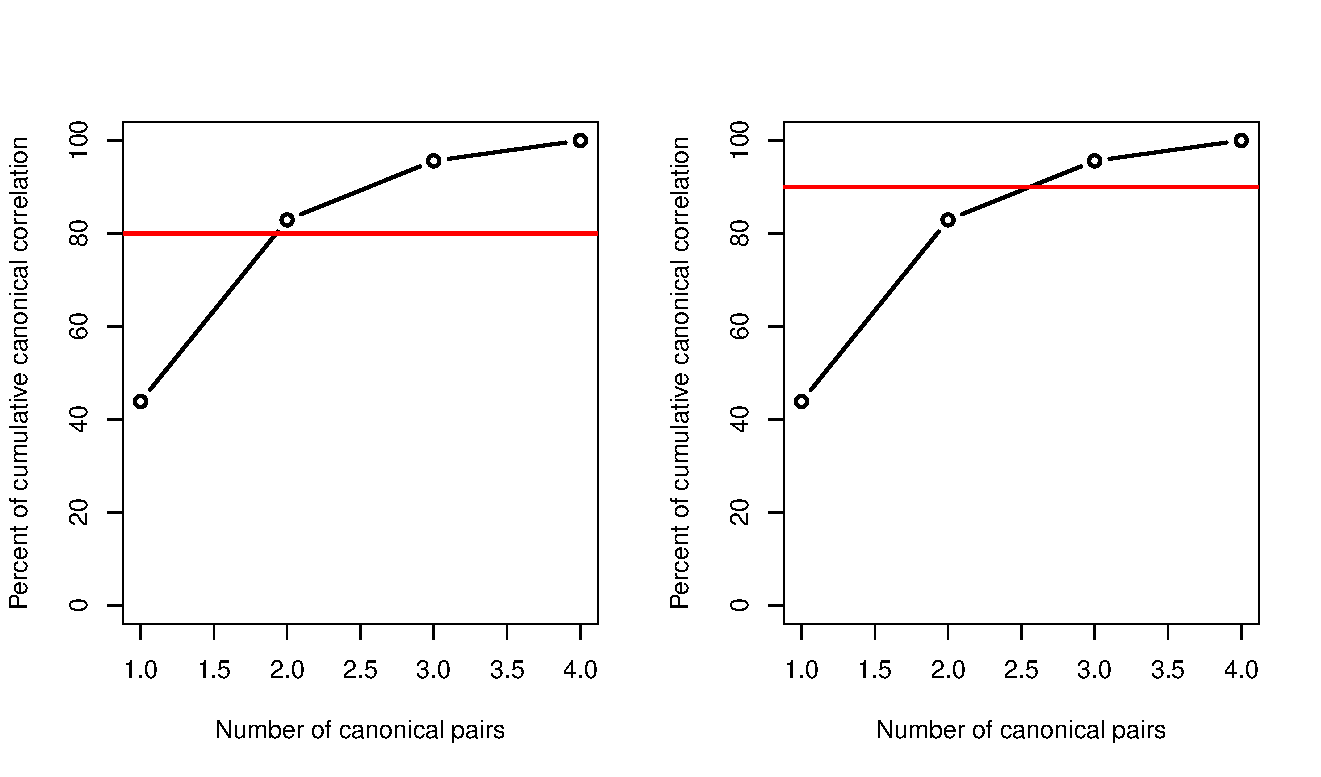
\includegraphics[width=12cm,height=6cm]{pulp_cor.pdf}
\vspace{-5mm}
\caption{Cumulative canonical correlation plot in pulp data in Section 3.2}
\label{cca}
\end{center}
\end{figure}
%
According to Figure \ref{cca}(a) and (b), with 80\% cumulative canonical correlations,
two canonical pairs are enough,
while three canonical pairs should be good with the default 90\%.
%%%%%%%%%%%%%%%%%%%%%%%%%%%%%%%%%%%%%%%%%%%%%%%%%%%%%%%%%%%%%%%%%%%%%%%%%%%%
%%%%%%%%%%%%%%%%%%%%%%%%%%%%%%%%%%%%%%%%%%%%%%%%%%%%%%%%%%%%%%%%%%%%%%%%%%%%

\subsection{Ordinary least squares: pulp data}
If the dimension of either $\mathbf{X}$ or $\mathbf{Y}$ is equal to one,
the estimated canonical coefficient matrix from the standard CCA
is equivalent to that from ordinary least squares.
In such case,  the command \code{seedCCA(X, Y[,1], type="cca")}  results in
the ordinary least squares estimate, which is ``seedols'' subclass.
The output of "seedols" has three components, which are  the estimated coefficients 
and the two sets of variables.
For example, assume that a regression study of arithmetic fiber length,
which is the first column of $\mathbf{Y}$, given $\mathbf{X}$ is of specific interest.
It should be noted that the order of \code{seedCCA(X, Y[,1], type="cca")}
and \code{seedCCA(Y[,1], X, type="cca")}  does not matter,
and any of them yields the same results.
Also, the commands of \code{coef(object)} and \code{fitted(object)} return
the estimated coefficients and fitted values from the ordinary least squares, respectively.
%Then its fitted value is essentially equivalent to
%\code{Xphi} obtained from \code{finalCCA} application
%for arithmetic fiber and $\mathbf{X}$.
%It can be confirmed from the R-codes below.
%Therefore, one needs to compute least squares in such situation,
%\textsf{seedCCA}-package can do it in free of charge.
%
\begin{verbatim}
## extracting arithmatic fiber from Y
> fit.ols <- seedCCA(X, Y[, 1], type="cca")
NOTE:  One of the two sets are 1-dimensional, so a linear regression via ordinary least
square is fitted.

> names(fit.ols)
[1] "coef"  "X"  "Y"

> coef(fit.ols)
> fitted(fit.ols)
\end{verbatim}
%

%%%%%%%%%%%%%%%%%%%%%%%%%%%%%%%%%%%%%%%%%%%%%%%%%%%%%%%%%%%%%%%%%%%%%%%%%%%%
%%%%%%%%%%%%%%%%%%%%%%%%%%%%%%%%%%%%%%%%%%%%%%%%%%%%%%%%%%%%%%%%%%%%%%%%%%%%
\subsection{Seeded CCA (case 1): {\sf cookie} data}
The biscuit dough data set called \code{cookie} in \pkg{seedCCA}
comes from the experiment of
analyzing the composition of biscuits by NIR spectroscopy.
Two sets of variables are obtained from 72 biscuit samples.
The first set of variables is wavelengths measured by spectroscopy.
In the original data set, wavelengths at 700 different points
from 1100 to 2798 nanometers (NM) at the steps of 2nm were measured.
However, since some of the figures seemed to contain little information,
wavelengths from 1380nm to 2400 at an interval of 4nm were analyzed.
The second set of variables is the percentages of
four ingredients: biscuits- fat, sucrose, dry flour, and water.
Since the 23rd and 61st samples
in the data set were believed to be outliers,
they were deleted from the data set.
The standard CCA is not applicable because of  $p=256>n=72$, and
case 1 of the seeded CCA should be fitted, considering that $n=72>>r=4$.

The basic command for this is \code{seedCCA(X, Y, type="seed1")},
which results in ``finalCCA'' subclass.
Regardless of the order of \code{X} and \code{Y},
the lower dimensional set alone is reduced in the initial step.
Therefore,  \code{seedCCA(X, Y, type="seed1")} and  \code{seedCCA(Y, X, type="seed1")}
basically produce the same seeded CCA results.
For \code{type="seed1"}, the values of the options of \code{ux}, \code{uy}, \code{u},
\code{eps}, and \code{AS} affect the implementation, whose defaults are
\code{NULL}, \code{NULL}, 10,  0.01, and \code{TRUE}, respectively.

Option \code{u} controls the maximum number of projections 
unless both \code{ux} and \code{uy} are specified.
The option \code{ux=k} works only when the dimension of the first set \code{X}
is bigger than that of the second set \code{Y}.
Then, the maximum number of projections becomes the value given in \code{ux=k}.
The option \code{uy} works in the opposite way to \code{ux}.
The options of  \code{AS=TRUE} and \code{eps} control
automatic termination of the projections before reaching the maximum given in
\code{u}, \code{ux}, or \code{uy}.
The projection is terminated if the increment gets less than the value given in \code{eps}.
Then, the first candidate value, which satisfies the stopping criteria,
is suggested as a proper value of projections.
If any of \code{ux}, \code{uy}, and \code{u} are specified not enough
to guarantee the automatic stopping,  a notice is provided to increase it.

After running \code{seedCCA(X, Y, type="seed1")}, a plot for the proper selection of \code{u} is
automatically constructed, and a blue vertical bar in the plot is the suggested value of \code{u}.
%
\begin{verbatim}
## loading cookie data
> data(cookie)
> myseq<-seq(141, 651, by=2)
> A <- as.matrix(cookie[-c(23, 61), myseq])
> B <- as.matrix(cookie[-c(23, 61), 701:704])

## seedec CCA with case 1
> fit.seed1.ab <- seedCCA(A, B, type="seed1") ## the first set A has been initial-CCAed.
NOTE:  Seeded CCA with case 1 is fitted. The set with larger dimension is initially reduced.
The first and second sets are denoted as X and Y, respectively.

> fit.seed1.ba <- seedCCA(B, A, type="seed1") ##  the second set A has been initial-CCAed.
NOTE:  Seeded CCA with case 1 is fitted. The set with larger dimension is initially reduced.
The first and second sets are denoted as X and Y, respectively.

> names(fit.seed1.ab)
[1] "cor"  "xcoef"  "ycoef"  "proper.u"  "initialMX0"  "newX" "Y"  "Xscores"  "Yscores"

> names(fit.seed1.ba)
[1] "cor"  "xcoef"  "ycoef"  "proper.u"  "X"  "initialMY0"  "newY"  "Xscores"  "Yscores"

> fit.seed1.ab$xcoef[, 3] <- -fit.seed1.ab$xcoef[, 3] ## changing the sign
> fit.seed1.ab$xcoef[, 4] <- -fit.seed1.ab$xcoef[, 4] ## changing the sign

> all(round(fit.seed1.ab$cor, 5)== round(fit.seed1.ba$cor, 5))
[1] TRUE

> fit.seed1.ab$proper.u
[1] 3

> fit.seed1.ba$proper.u
[1] 3

> all(round(fit.seed1.ab$xcoef, 5) == round(fit.seed1.ba$ycoef, 5))
[1] TRUE

> fit.seed1.ab.ux <- seedCCA(A, B, type="seed1", ux=2)
The maximum number of iterations is reached. So, users must choose u bigger than 2.

> fit.seed1.ab.ux$proper.u
[1] 2
\end{verbatim}
%
For \code{fit.seed1.ab}, the first set \code{A} is reduced in the initial step.
The output component \code{initialMX0} is the estimate of ${\mathbf{M}}_{x,u_1}^{0}$ 
and \code{newX} is ${\hat{\mathbf{M}}}_{x,u_1}^{0~{\rm T}}\mathbf{X}$.
On the contrary, in case of \code{fit.seed1.ba}, the second set \code{A}
is initially reduced, so \code{initialMY0} and \code{newY} are produced.
So, it is observed that the canonical correlations and suggested values of \code{u} from
 \code{fit.seed1.ab} and  \code{fit.seed1.ba} are equal,
not to mention that \code{fit.seed1.ab\$xcoef}  and \code{fit.seed1.ba\$ycoef} are the same.
The selection plot for \code{u} is reported in Figure \ref{data1u}, and
three projections are suggested.
Since \code{ux} is not given big enough in \code{seedCCA(A, B, type="seed1", ux=2)},
the following warning is given:
\begin{verbatim}
The maximum number of iterations is reached. So, users must choose u bigger than 2.
\end{verbatim}
%
\begin{figure}\begin{center}
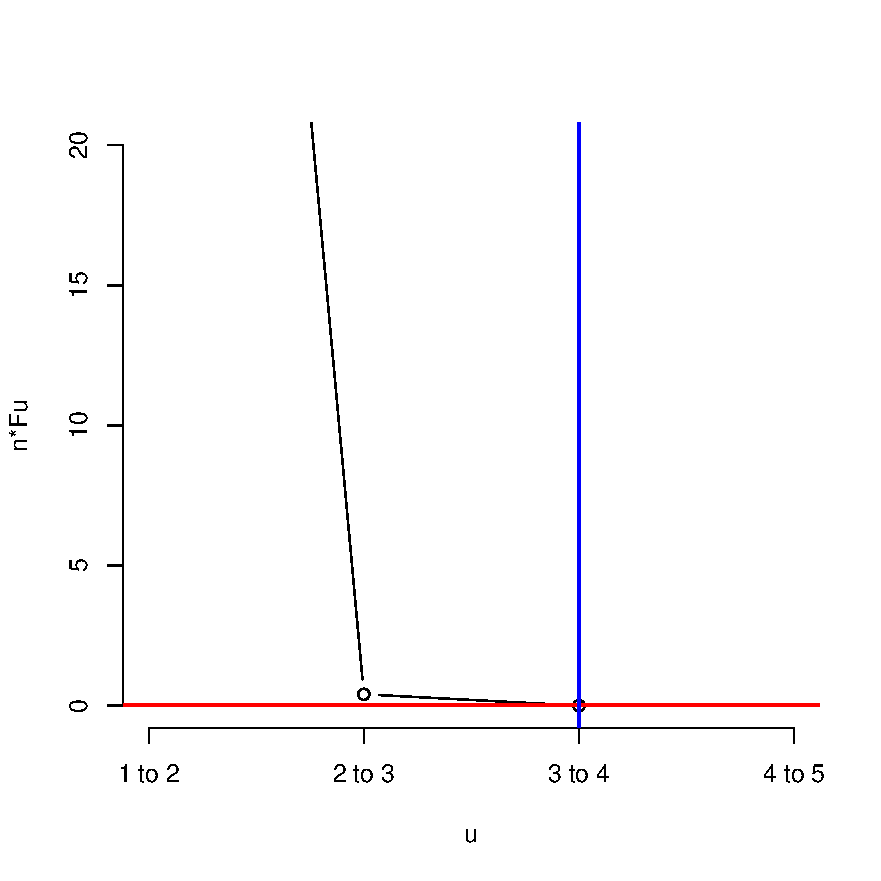
\includegraphics[width=6cm,height=6cm]{data1u.pdf}
\vspace{-5mm} \caption{Selection plot of \code{u}  generated from
\code{seedCCA(A, B, type="seed1")} in Section 3.4}
\label{data1u}
\end{center}\end{figure}
%

Next, we change the values of \code{ux}, \code{uy}, \code{AS}, and \code{eps}.
Since the usage of these options for \code{type="seed1"} are the same as
that for \code{type="seed2"} and \code{type="pls"}.
To measure the computing time, the \pkg{tictoc} package (\cite{tictoc}) is used
with Intel(R) Core(TM)i7 2.9GHz and 12GB Ram computer.
%
\begin{verbatim}
> seedCCA(A, B, type="seed1", ux=5)$proper.u
[1] 3

> seedCCA(B, A, type="seed1", eps=0.000001)$proper.u
[1] 4

> library(tictoc)
> tic()
> seedCCA(B, A, type="seed1", u=30)$proper.u
> toc()
0.03 sec elapsed

> tic()
> seedCCA(B, A, type="seed1", u=30, AS=FALSE)$proper.u
> toc()
0.29 sec elapsed
\end{verbatim}
%
Usage of \code{AS} should be noted. With bigger choices of \code{u} and \code{AS=FALSE},
the running time of the function will be longer.
%%%%%%%%%%%%%%%%%%%%%%%%%%%%%%%%%%%%%%%%%%%%%%%%%%%%%%%%%%%%%%%%%%%%%%%%%%%%
%%%%%%%%%%%%%%%%%%%%%%%%%%%%%%%%%%%%%%%%%%%%%%%%%%%%%%%%%%%%%%%%%%%%%%%%%%%%
\subsection{Seeded CCA (case 2) versus Regularized CCA: {\sf nutrimouse} data}
The nutrimouse data was collected
from a nutrition study in 40 mice $(n=40)$.
One of two sets of variables was expressions of
120 genes measured in liver cells by microarray technology.
The other set of variables was concentrations of
21 hepatic fatty acids(FA) measured through gas chromatography.
In addition, the forty mice are
cross-classified based on two factors, genotype and diet.
There are two genotypes, wild-type (WT) and
PPAR$\alpha$ deficient (PPAR$\alpha$) mice and five diets: 
corn and colza oils (50/50 REF),
hydrogenated coconut oil for a saturated FA diet (COC),
sunflower oil for $\omega$6 FA-rich diet (SUN),
linseed oil for $\omega$3-rich diet (LIN) and
corn/colza/enriched fish oils (42.5/42.5/15, FISH).
The nutrimouse data is contained in the \pkg{seedCCA} package.

In this data, case 2 of the seeded CCA should be used 
because $\min(120,21)$ is relatively big compared to $n=40$.
Then, case 2 of the seeded CCA requires to choose
how many eigenvectors of $\hat{\boldsymbol \Sigma}_{xy}$
should be enough to replace it.
%$\hat{\boldsymbol \Sigma}_{xy}$ .
This is another tuning parameter for case 2 of the seeded CCA
along with the number of projections.
The option \code{cut} in \code{seedCCA} controls automatic selection
of the number of  eigenvectors of $\hat{\boldsymbol\Sigma}_{xy}$.
The option \code{cut=$\alpha$} determines a set of the eigenvectors
whose cumulative proportions of their corresponding eigenvalues
is bigger than equal to $\alpha$.
For the set of eigenvectors to be chosen conservatively,
we set the default of \code{cut} at 0.9.
Also, users can directly give the number of eigenvectors
using \code{d}. Unless \code{d} is \code{NULL}, the option \code{cut} is discarded.
This means that \code{cut} works only when \code{d=NULL}.
If users want to use \code{d}, then a function \code{covplot} should be run first.
The function \code{covplot} has the option \code{mind},
which set the number of the eigenvalues to show their cumulative percentages.
Its default is \code{NULL}, and then it becomes $\min(p,r)$.
The function returns the eigenvalues, the cumulative percentages, 
and the number of the eigenvectors to account for 
60\%, 70\%, 80\%, and 90\% of the total variation
along with the scree plot of the eigenvalues.

The results of the seeded and regularized CCAs are compared.
Since the regularized CCA is necessary to choose proper values of the two parameters,
we compare running times for the automatic searches for
the regularized and seeded CCAs via the \pkg{tictoc} package.
For \pkg{seedCCA}, we use the default value of \code{cut}.
%
\begin{verbatim}
> library(CCA)
> library(tictoc)

## loading nutrimouse data
> data(nutrimouse)
> X <- scale(as.matrix(nutrimouse$gene))
> Y <- scale(as.matrix(nutrimouse$lipid))

## determining the number of the eigenvectors of cov(X,Y) with cut=0.9
> tic("SdCCA")
> fit.seed2 <- seedCCA(X, Y)
> toc()
SdCCA: 0.13 sec elapsed

## finding the optimal values of lambda1 and lambda2 for RCCA
> tic("Regularized CCA")
> res.regul <- estim.regul(X, Y, plt=TRUE, grid1=seq(0.0001, 0.2, l=51), grid2=seq(0, 0.2, l=51))
> toc()
Regularized CCA 819.58 sec elapsed

## scree plot of cov(X, Y)
> names(covplot(X, Y, mind=10))
[1] "eigenvalue"  "cum.percent" "num.evecs"

> names(fit.seed2)
[1] "cor"  "xcoef"  "ycoef"  "proper.ux"  "proper.uy"  "d"  "initialMX0"  "initialMY0"
[9] "newX"  "newY"  "Xscores"    "Yscores"

> fit.seed2$d
[1] 3
\end{verbatim}
%
%
\begin{figure}\begin{center}
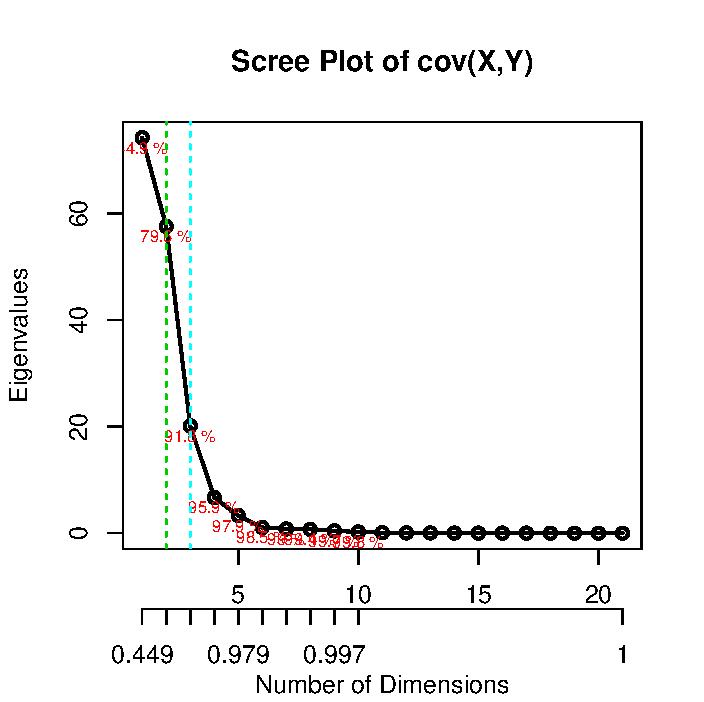
\includegraphics[width=6cm,height=6cm]{data2cov10s.pdf}
\vspace{-3mm}\caption{Scree plots for the selection of
sets of eigenvectors to replace $\rm{cov}(\mathbf{X}, \mathbf{Y})$
generated from \code{covplot(X, Y, mind=10)}  in Section 3.5}
\label{data2cov}
\end{center}\end{figure}
%
Since \code{type="seed2"} reduces the dimensions of \code{X} and \code{Y}
at the initialized CCA step, the output components of
\code{initialMX0}, \code{initialMY0}, \code{newX} and \code{newY} and \code{d}
are reported.

The plot generated from \code{covplot(X, Y, mind=10)} is given in Figure \ref{data2cov}.
According to Figure \ref{data2cov},
the first two, three, and four eigenvalues account for
79.6\%, 91.8\%, and 95.9\% of the total variation of
$\hat{\boldsymbol{\Sigma}}_{xy}$, respectively.
Using 90\% conservative guideline,  it is determined that
the first three largest eigenvectors replace $\hat{\boldsymbol{\Sigma}}_{xy}$ well enough.

The selection plot of \code{ux} and \code{uy} is given in Figure \ref{data2uxuy}.
The figure suggests that $u_x$ and $u_y$ are equal to 7 and 6, respectively.
%
\begin{figure}\begin{center}
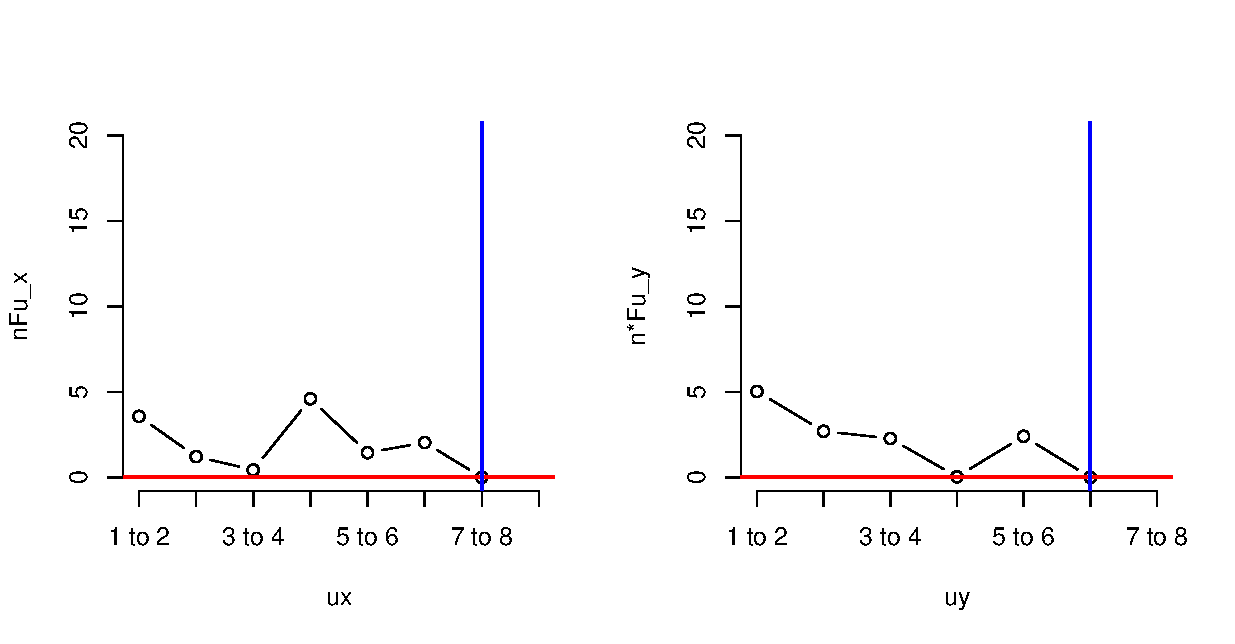
\includegraphics[width=12cm,height=6cm]{data2uxuy3.pdf}
\vspace{-5mm}\caption{Selection plot of \code{ux}  and \code{uy} generated from
\code{seedCCA(X, Y)} in Section 3.5}
\label{data2uxuy}
\end{center}\end{figure}
%

Now we compare the parameter selection time.
For the regularized CCA, it can be done with \code{estim.regul}, and
users must provide a small enough range for them to reduce the computing time.
The resulted optimal $\lambda_1$ and $\lambda_2$ are 0.168016 and 0.004, respectively.
With Intel(R) Core(TM)i7 2.9GHz and 12GB Ram,
the seeded CCA took 0.32 seconds,
while 819.58 seconds, around 13.5 minutes, lapsed for the regularized CCA.
This difference is really huge,
so time consumed in the selection of \code{ux}, \code{uy} and, \code{d}
is trivially small compared to the regularized CCA.
This is a clear desirable aspect and advantage of the seeded CCA over the regularized one.

Next, we compare the first two pairs of estimated canonical variates.
The results shown in Figures \ref{fpair}--\ref{spair} are
equivalent to the analysis discussed in \cite{ecca}.
%
\begin{verbatim}
## Extracting the first two pairs of canonical variates
> sx1 <- fit.seed2$Xscores[, 1]
> sx2 <- fit.seed2$Xscores[, 2]
> sy1 <- fit.seed2$Yscores[, 1]
> sy2 <- fit.seed2$Yscores[, 2]

## fitting the regularized CCA
> res.rcc <- rcc(X, Y, 0.168016, 0.004)
> RCCA.X <- X%*%res.rcc$xcoef
> RCCA.Y <- Y%*%res.rcc$ycoef
> rx1 <- RCCA.X[,1]
> rx2 <- RCCA.X[,2]
> ry1 <- RCCA.Y[,1]
> ry2 <- RCCA.Y[,2]

par(mfrow=c(1,2))
> with(plot(rx1, ry1, col=c(2,4)[genotype], pch=c(1,2)[genotype],
+ main="1st pair from RCCA", xlab="rx1", ylab="ry1"), data=nutrimouse)
> with(legend(-1.4, 1.4, legend=levels(genotype), col=c(2,4), pch=c(1,2), cex=1.5),
+ data=nutrimouse)
> with(plot(-sx1, -sy1, col=c(2,4)[genotype], pch=c(1,2)[genotype],
+ main="1st pair from seedCCA", xlab="sx1", ylab="sy1"), data=nutrimouse)
> with(legend(-1.5, 1.6, legend=levels(genotype), col=c(2,4), pch=c(1,2), cex=1.5),
+ data=nutrimouse)

> par(mfrow=c(1,2))
> with(plot(rx2, ry2, col=c(1:4,6)[diet], pch=c(15,16,17,18,20)[diet], cex=1.5,
+ main="2nd pair from RCCA", xlab="rx2", ylab="ry2"), data=nutrimouse)
> with(legend(-2.3, 1.9, legend=levels(diet), col=c(1:4,6), pch=c(15:18,20)),
+ data=nutrimouse)
> with(plot(sx2, sy2, col=c(1:4,6)[diet], pch=c(15,16,17,18,20)[diet], cex=1.5,
+ main="2nd pair from seedCCA", xlab="sx2", ylab="sy2"), data=nutrimouse)
with(legend(-2.5, 1.9, legend=levels(diet), col=c(1:4,6), pch=c(15:18,20)),
+ data=nutrimouse)
\end{verbatim}

%
\begin{figure}\begin{center}
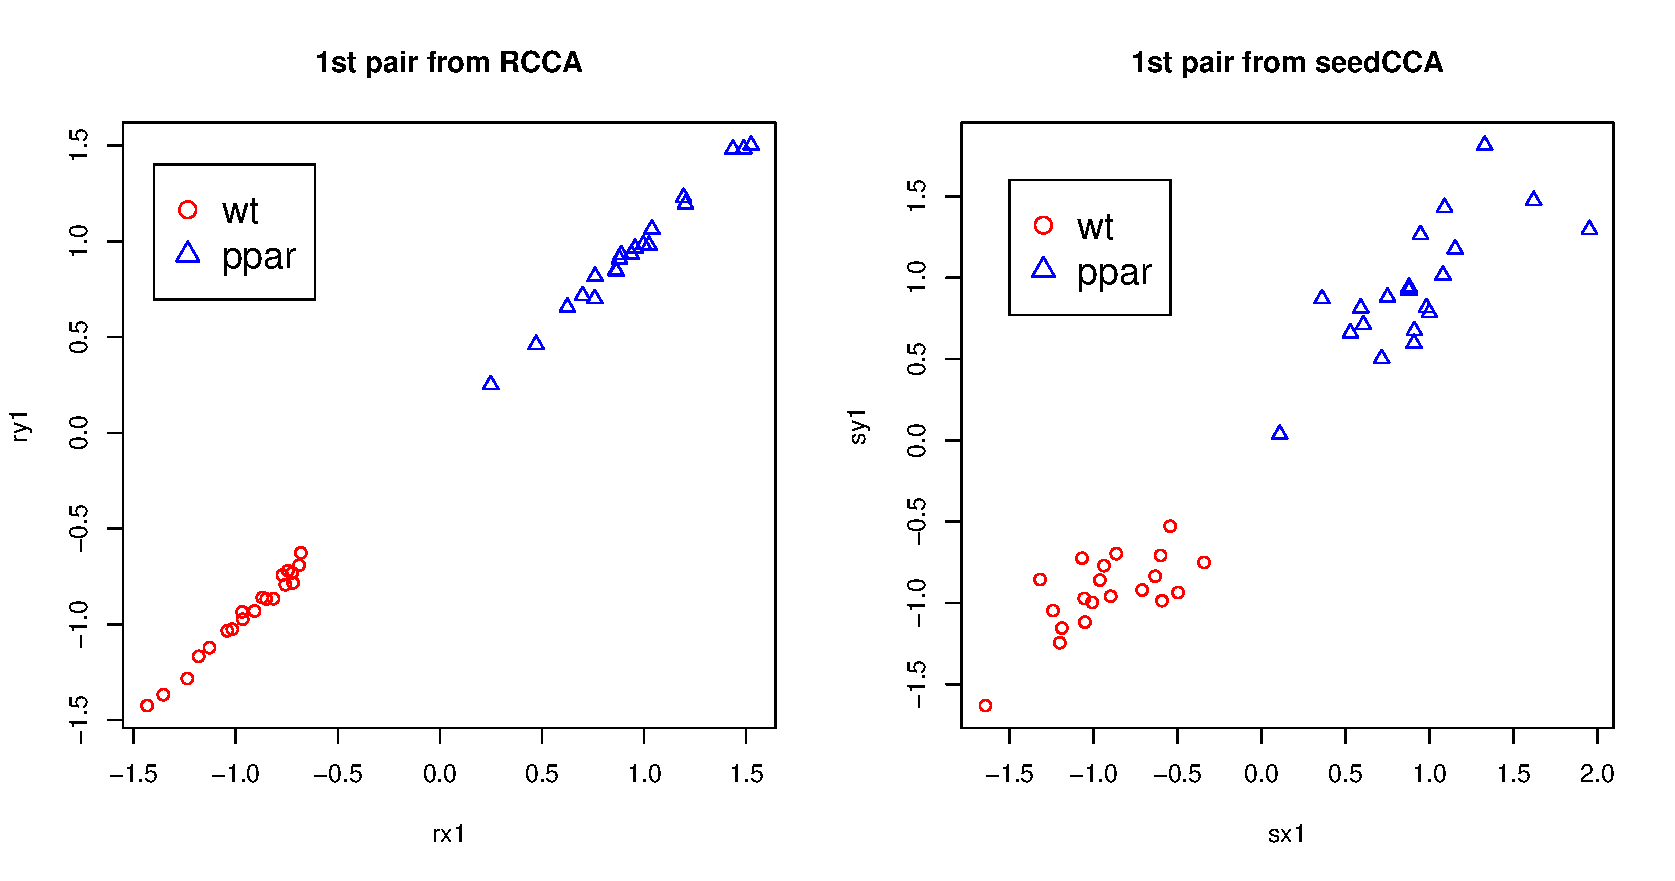
\includegraphics[width=12cm,height=6cm]{1stpair.pdf}
\vspace{-5mm}\caption{the first pair of canonical variates
from regularized CCA  and seeded CCA marked with genotype in Section 3.5}
\label{fpair}
\end{center}\end{figure}
%
\begin{figure}\begin{center}
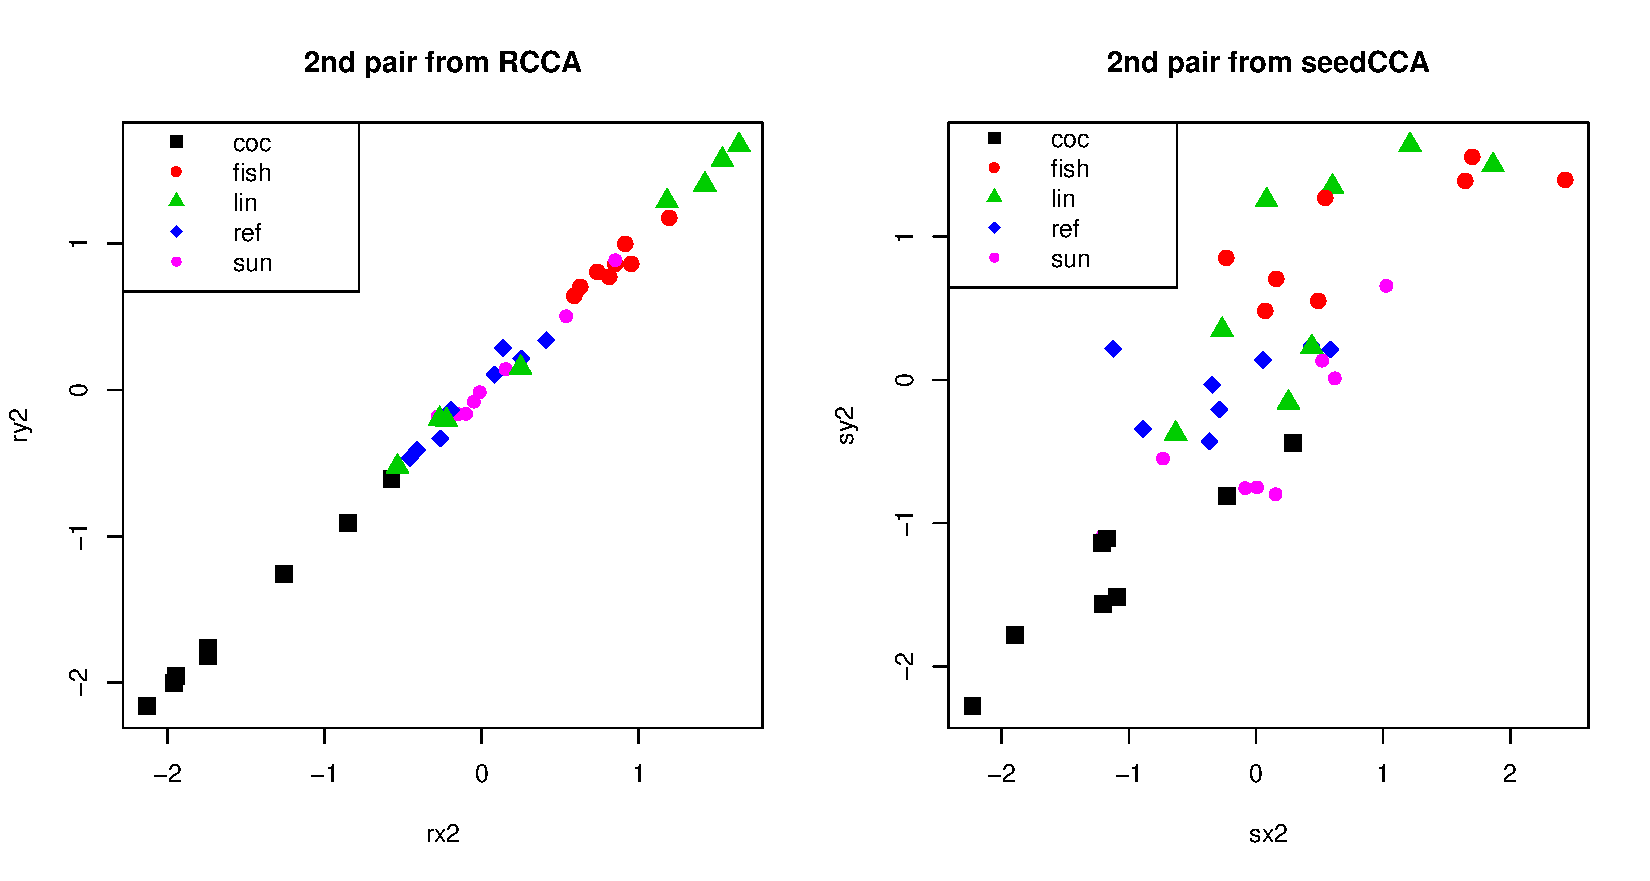
\includegraphics[width=12cm,height=6cm]{2ndpair.pdf}
\vspace{-5mm}\caption{the second pair of canonical variates
from regularized CCA  and seeded CCA marked with diet in Section 3.5}
\label{spair}
\end{center}\end{figure}
%

According to Figures \ref{fpair}--\ref{spair},
the first pair of canonical variates from both CCAs
distinguish genotype very well,
but their second pairs marked with diet are quite complex.
To have more insight into the results for the second pair on a diet,
multivariate analysis of variance is fitted. 
Further pairwise comparison is done via \pkg{lsmeans} (\cite{lsmeans})
with level 5\% and $p$-values adjusted by false discovery rate \cite{fdr}.
%
\begin{verbatim}
> library(lsmeans)
> fit2r <- manova(cbind(rx2, ry2)~diet, data=nutrimouse)
> fit3sd <- manova(cbind(sx2, sy2)~diet, data=nutrimouse)
> test( contrast( lsmeans(fit2r, "diet"), "pairwise"), side = "=",  adjust = "fdr")
 contrast     estimate        SE df t.ratio p.value
 coc - fish -2.3842686 0.2684019 35  -8.883  <.0001
 coc - lin  -2.1749708 0.2684019 35  -8.103  <.0001
 coc - ref  -1.4881111 0.2684019 35  -5.544  <.0001
 coc - sun  -1.6582635 0.2684019 35  -6.178  <.0001
 fish - lin  0.2092978 0.2684019 35   0.780  0.4897
 fish - ref  0.8961575 0.2684019 35   3.339  0.0040
 fish - sun  0.7260051 0.2684019 35   2.705  0.0175
 lin - ref   0.6868597 0.2684019 35   2.559  0.0214
 lin - sun   0.5167073 0.2684019 35   1.925  0.0780
 ref - sun  -0.1701524 0.2684019 35  -0.634  0.5302

Results are averaged over the levels of: rep.meas
P value adjustment: fdr method for 10 tests

> test( contrast (lsmeans(fit3sd, "diet"), "pairwise"), side = "=",  adjust = "fdr")
 contrast      estimate        SE df t.ratio p.value
 contrast      estimate        SE df t.ratio p.value
 coc - fish -2.14838660 0.3163067 35  -6.792  <.0001
 coc - lin  -1.79396325 0.3163067 35  -5.672  <.0001
 coc - ref  -1.07697196 0.3163067 35  -3.405  0.0035
 coc - sun  -1.03303440 0.3163067 35  -3.266  0.0041
 fish - lin  0.35442334 0.3163067 35   1.121  0.3001
 fish - ref  1.07141463 0.3163067 35   3.387  0.0035
 fish - sun  1.11535219 0.3163067 35   3.526  0.0035
 lin - ref   0.71699129 0.3163067 35   2.267  0.0371
 lin - sun   0.76092885 0.3163067 35   2.406  0.0308
 ref - sun   0.04393756 0.3163067 35   0.139  0.8903

Results are averaged over the levels of: rep.meas
P value adjustment: fdr method for 10 tests
\end{verbatim}
%
For the regularized CCA, the ``coc'' diet is different from the others. 
Moreover ``fish'' differs from ``sun''.
However, the other pairwise comparisons are quite mixed.
It is determined that there are no significant differences between
``fish-lin'', ``lin-sun'', and ``ref-sun''.
On the contrary, reasonable pairwise comparison results come
from the seeded CCA.
Like the others, the ``coc'' diet is different from the others.
Furthermore, ``fish-lin'' is not significantly different, and
``ref-sun'' is concluded to be similar.
Fish oil is known to contain $\omega 3$, and linseed oil is designed for it.
Therefore, this conclusion would be reasonable.
Also, the reference oil diet consists of corn and colza oil,
which is known to contain $\omega 6$.
Since sun-flower oil is, indeed, for $\omega 6$-rich diet,
this result is also reasonable.
In this regard, the seeded CCA results would be preferable to the regularized CCA.

%%%%%%%%%%%%%%%%%%%%%%%%%%%%%%%%%%%%%%%%%%%%%%%%%%%%%%%%%%%%%%%%%%%%%%%%%%%%
%%%%%%%%%%%%%%%%%%%%%%%%%%%%%%%%%%%%%%%%%%%%%%%%%%%%%%%%%%%%%%%%%%%%%%%%%%%%

\subsection{Partial least square application with {\sf nutrimouse} data}
With the nutrimouse data, consider a regression of the first one, `` C14.0''
in concentrations of 21 hepatic fatty acids given expressions
of 120 genes measured in liver cells.
In this case, partial least squares is a front-runner choice.
Then, to obtain the partial least square estimator in \pkg{seedCCA},
one needs to implement \code{seedCCA(X, Y, type="pls")}.
This results in ``seedpls'' subclass.
An important matter in partial least squares is
that the first set of the variable must be predictors.
The response variable can be either univariate or multivariate.
Option \code{u} is recommended to set reasonably small 
because the estimated coefficients are reported up to
the value given in \code{u}.
If \code{scale=TRUE}, the predictors are standardized
to have zero sample means and the sample correlation matrix.

The estimated coefficients and fitted values by partial least square can be obtained
via \code{coef(object, u=NULL)} and \code{fitted(object, u=NULL)}.
The default of \code{u} in both \code{coef} and \code{fitt} is \code{NULL}.
In both functions, usage of \code{u} is equivalent.
If \code{u=k} is specified,  only the estimated coefficients and fitted values
computed from \code{k} projections are reported.
All of the coefficient estimates and fitted values are reported up to  \code{u},
if \code{u=NULL}.

For \code{type="pls"}, the automatic procedure to suggest
a proper value of projections is not conducted.
For the ``seedpls'' subclass, \code{plot(object)} suggests a proper value of projections
along with other output components.
If the terminating condition is not satisfied before reaching the value of \code{u},
then  \code{plot(object)} provides a caution to increase the value of \code{u}.
%
\begin{verbatim}
> data(nutrimouse)
> Y <- as.matrix(nutrimouse$lipid)
> X <- as.matrix(nutrimouse$gene)
> Y1 <- as.matrix(Y[, 1])  ## univariate response
> Y12 <- as.matrix(Y[, 1:2])  ## multivariate response

## fitting partial least square and obtaining the estimated coefficient vector
> fit.pls1.10 <- seedCCA(X, Y1, u=10, type="pls")
> fit.pls1.3 <- seedCCA(X, Y1, u=3, type="pls", scale=TRUE)

> names(fit.pls1.10)
[1] "coef"  "u"     "X"     "Y"     "scale"

> names(fit.pls1.10$coef)
[1] u=1"  "u=2"  "u=3"  "u=4"  "u=5"  "u=6"  "u=7"  "u=8"  "u=9"  "u=10"

> names(fit.pls1.3$coef)
[1] "u=1" "u=2" "u=3"

> fit.pls1.3$scale
[1] TRUE

> par(mfrow=c(1,2))
> plot(fit.pls1.10)
$proper.u
[1] 6
$nFu
[1] 6.344725e+00 2.383108e+00 1.681329e+00 2.669394e+00 1.853061e+00 3.217472e-04 5.296046e-05
[8] 6.017641e-06 4.895905e-07 3.117371e-08
$u
[1] 10
$eps
[1] 0.01
> title("fit.pls1.10")

> plot(fit.pls1.3)
Caution: The terminating condition is NOT satisfied. The number of projections should be bigger than  3.
$proper.u
[1] 3
$nFu
[1] 6.344725 2.383108 1.681329
$u
[1] 3
$eps
[1] 0.01
> title("fit.pls1.3")

> names(fitted(fit.pls1.10))
[1] "u=1"  "u=2"  "u=3"  "u=4"  "u=5"  "u=6"  "u=7"  "u=8"  "u=9"  "u=10"

> fitted(fit.pls1.10, u=6)
     1      2      3      4      5      6      7      8      9     10     11     12     13     14
 0.137  0.368  0.317  0.346  0.492  1.620  0.722  0.003  0.065  1.212  0.458  0.640  0.272  0.397
    15     16     17     18     19     20     21     22     23     24     25     26     27     28
-0.103  0.426  1.448  0.287  1.264  0.517  2.803  0.914  0.043  0.028  0.234  0.598  0.875  0.434
    29     30     31     32     33     34     35     36     37     38     39     40
 0.694  0.666  2.958  2.350  0.620  0.958  0.495  2.790  0.701  0.168  0.767  0.535

> fit.pls.m <- seedCCA(X, Y12, u=5, type="pls")
> dim(fit.pls.m$coef$'u=1')
[1] 120   2
\end{verbatim}
%
\begin{figure}\begin{center}
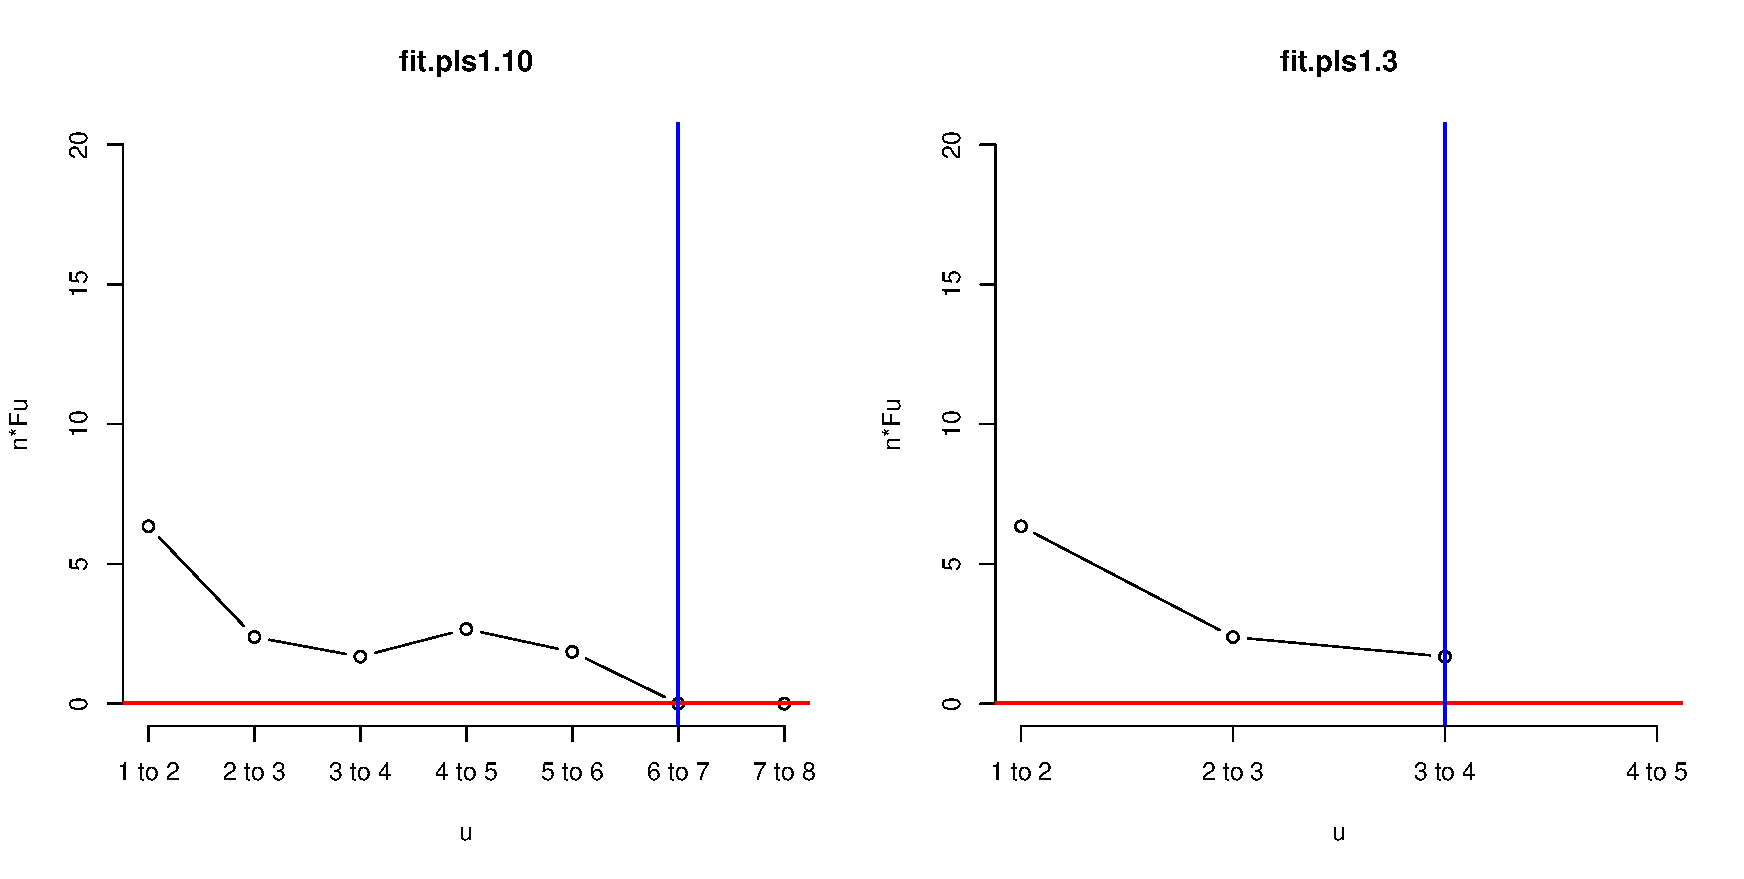
\includegraphics[width=12cm,height=6cm]{pls_selu.pdf}
\vspace{-5mm}\caption{Selection plot of \code{u}  generated from
\code{seedCCA(X, Y1, u=10, type="pls")}(left) and
\code{seedCCA(X, Y1, u=3, type="pls", scale=TRUE)}(right)
 in Section 3.6}
\label{pls_selu}
\end{center}\end{figure}
%

The selection of projections for two partial least squares by
\code{seedCCA(X, Y1, u=10, type="pls")} and
\code{seedCCA(X, Y1, u=3, type="pls", scale=TRUE)}
is given in Figure \ref{pls_selu}.
According to Figure \ref{pls_selu}, the proper value of projection is suggested at 6
for \code{fit.pls1.10} object, while the termination condition is not satisfied  for \code{fit.pls1.3} object,
so a caution statement is given.

%%%%%%%%%%%%%%%%%%%%%%%%%%%%%%%%%%%%%%%%%%%%%%%%%%%%%%%%%%%%%%%%%%%%%%%%%%%%
%%%%%%%%%%%%%%%%%%%%%%%%%%%%%%%%%%%%%%%%%%%%%%%%%%%%%%%%%%%%%%%%%%%%%%%%%%%%
%%%%%%%%%%%%%%%%%%%%%%%%%%%%%%%%%%%%%%%%%%%%%%%%%%%%%%%%%%%%%%%%%%%%%%%%%%%%
%%%%%%%%%%%%%%%%%%%%%%%%%%%%%%%%%%%%%%%%%%%%%%%%%%%%%%%%%%%%%%%%%%%%%%%%%%%%

\section{Discussion}
When a study between two sets of variables,
saying $(\mathbf{X}\in\mathbb{R}^{p}, \mathbf{Y}\in\mathbb{R}^{r})$,
is of primary interest,
canonical correlation analysis (CCA; \cite{cca}) is still
popularly used in explanatory studies.
The CCA has successful application in many science fields
such as chemometrics, pattern recognition, genomic sequence analysis, and so on.

The recently developed \pkg{seedCCA} package implements
a collection of CCA methodologies
including the standard CCA application, seeded CCA, and partial least squares.
The package enables us to fit CCA to large-$p$ and small-$n$ data.
The paper provides a complete guide for
the package to implement all the methods, along with three real data examples.
Also, the seeded CCA application results are compared
with the regularized CCA in the existing \pkg{CCA} package.

It is believed that the package, along with the paper, 
will contribute to high-dimensional data analysis
in various scientific field practitioners and
that the statistical methodologies in multivariate analysis
become more fruitful.
%%%%%%%%%%%%%%%%%%%%%%%%%%%%%%%%%%%%%%%%%%%%%%%%%%%%%%%%%%%%%%%%%%%%%%%%%%%%
%%%%%%%%%%%%%%%%%%%%%%%%%%%%%%%%%%%%%%%%%%%%%%%%%%%%%%%%%%%%%%%%%%%%%%%%%%%%
%%%%%%%%%%%%%%%%%%%%%%%%%%%%%%%%%%%%%%%%%%%%%%%%%%%%%%%%%%%%%%%%%%%%%%%%%%%%
%%%%%%%%%%%%%%%%%%%%%%%%%%%%%%%%%%%%%%%%%%%%%%%%%%%%%%%%%%%%%%%%%%%%%%%%%%%%
\section{Acknowledgments}
For the corresponding author Jae Keun Yoo,
this work was supported by Basic Science Research
Program through the National Research Foundation of Korea (NRF)
funded by the Korean Ministry of Education
(NRF-2019R1F1A1050715).
For Bo-Young Kim, this work
was supported by the BK21 Plus Project through the National
Research Foundation of Korea (NRF) funded by the Korean Ministry
of Education (22A20130011003).

\bibliography{yoo}

\address{Bo-Young Kim, Researcher\\
Celltrion\\
Incheon, 22014\\
Republic of Korea}

\address{Yunju Im, Postdoctoral Associate\\
Department of Biostatistics, Yale University\\
New Haven, CT 06520\\
United States of America}

\address{Jae Keun Yoo, Professor\\
Department of Statistics, Ewha Womans University\\
Seoul, 03760\\
Republic of Korea\\
\email{peter.yoo@ewha.ac.kr}}
